\section{Experimental Evaluation} \label{sec:experiments}

This section presents our experimental evaluation using a 12-node Linux cluster (kernel 3.10) and Apache Spark 2.4. Each node has 9 cores (each core is an Intel Xeon CPU at 1.70GHz) and 2G memory.

\textbf{Evaluation datasets}.
The details of the real datasets of polygons that we use are summarized in Table \ref{tab:datasets}. The first dataset (MainUS) contains the complete Census Tracts for all the states in the US mainland for years 2000 (layer A) and 2010 (layer B). 
It was collected from the official website of the United States Census Bureau\footnote{\url{https://www2.census.gov/geo/tiger/TIGER2010/TRACT/}}.  
The data was clipped to select just the states inside the continent. 
Something to note with this dataset is that the two layers  present a spatial gap (which was due to improvements in the precision introduced for 2010). As a result, there are considerably many more intersections between the two layers thus creating many new faces for the DCEL.

The second dataset (GADM - taken from Global Administration Areas\footnote{\url{https://gadm.org/}}) collects geographical boundaries of the countries and their administrative divisions around the globe.  
For our experiments, one layer selects the States (administrative level 2) and the other layer has the Counties (administrative  level 3).  
Since GADM may contain multi-polygons, we split them into their individual polygons. 

Since these two datasets are too large, a third, smaller dataset was created for comparisons with the sequential algorithm. This dataset is
the California Census Tracts (CCT) which is a subset from MainUS for the state of California; layer A corresponds to the CA census tracts from year 2000 while layer B for 2010. (Below we also use other states to create datasets with different number of faces).


\begin{table}
    \centering
    \ssp
    \small
    \caption{Evaluation Datasets}
    \label{tab:datasets}
    \begin{tabular}{c c c c}
        \toprule
        Dataset & Layer & Number        & Number    \\
                &       & of polygons   & of edges  \\
        \midrule
        MainUS& Polygons for 2000 & 64983 & 35417146        \\
              & Polygons for 2010 & 72521 & 36764043        \\
        GADM  & Polygons for Level 2 & 116995 & 32789444    \\
              & Polygons for Level 3 & 117891 & 37690256    \\
        CCT   & Polygons for 2000 & 7028 & 2711639          \\
              & Polygons for 2010 & 8047 & 2917450          \\
        \bottomrule
    \end{tabular}
\end{table}

\subsection{Overlay face optimizations}
We first examine the optimizations in Section \ref{sec:optimizing}. To consider different distributions of faces, for these experiments we used 8 states from the MainUS dataset with different number of tracks (faces). In particular, we used (in decreasing order of number of tracks): CA, TX, NC, TN, GA, VA, PA and FL. For each state we computed the distributed overlay between two layers (2000 and 2010). For each computation we compared the baseline (master at the root node) with intermediate reducers at different levels: $i$ varied from 4 to 10. 
Figure \ref{fig:overlay_tester} shows the results for the distributed overlay computation stage (that is, after the local DCELs were computed at each cell). Note that for each state experiment we tried different number of leaf cells for the quadtree and present the one with the best performance. 
As expected there is a trade-off between parallelism and how much work is left to the final reduce job. For different states the optimal $i$ varied between level 4 and 6.
The same figure also shows the optimization that re-partitions the faces by label id. This approach has actually the best performance. This is because there are few faces with the same label that can be combined independently. This results to smaller jobs that are better distributed among the cluster nodes and no reduce phase is needed. 
As a result, for the rest of the experiments we use the label re-partition approach to implement the overlay computation stage.

\begin{figure}
    \centering
    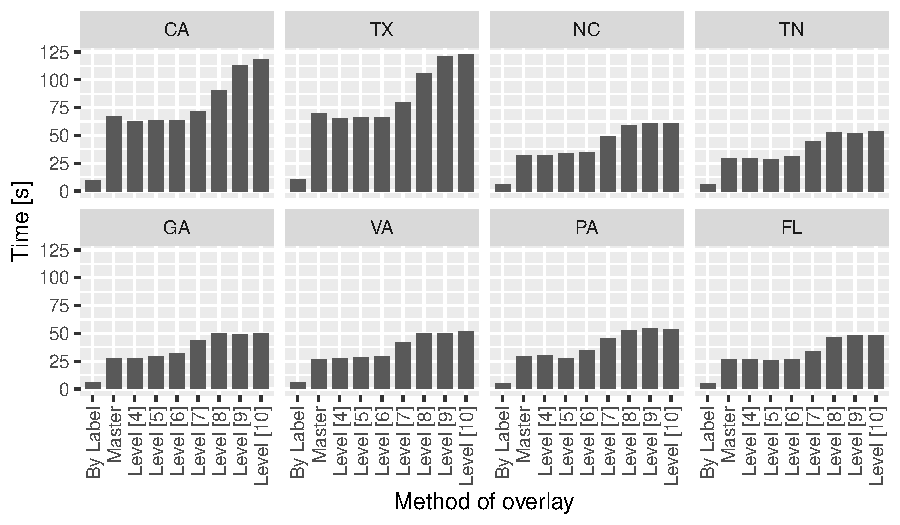
\includegraphics[width=0.8\linewidth]{figures/experiments/Overlay_Tester}
    \caption{Overlay methods evaluation.}\label{fig:overlay_tester}
\end{figure}

\subsection{Unbalanced layers optimization}

For these experiments we compared the traditional sweep approach with the `filtered-sweep' approach that considers only the areas where the smaller layer has edges (Section \ref{sec:unbalance}). 
To create the smaller cell layer, we picked a reference point in the state of Pennsylvania (from the MainUS dataset) and started adding 2000 census tracks until the number of edges reached 3K. We then varied the size of the larger cell layer in a controlled way: using the same reference point but using data from the 2010 census, we started adding tracks to create a layer that had around 2x, 3x, ..., 7x the number of edges of the smaller dataset. Since this optimization occurs per cell, we used a single node to perform the overlay computation within that cell.
Figure \ref{fig:unbalance_a} shows the behaviour of the two methods (filtered-sweep vs. traditional sweep) under the above described data for the overlay computation stage.  

Clearly, as the data from one layer grows much larger that the other layer the filtered-sweep approach overcomes the traditional one.

\begin{figure*}
    \centering
    \subfloat[\label{fig:unbalance_a}]{%
        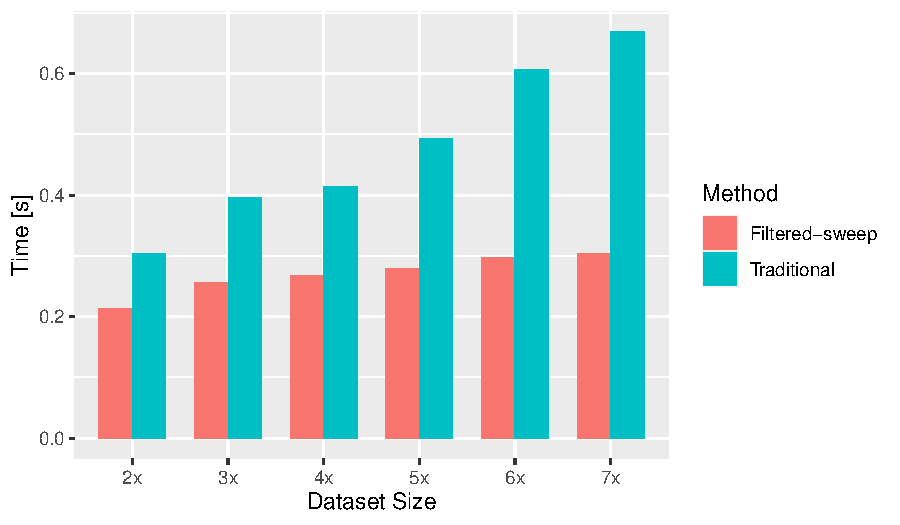
\includegraphics[width=0.48\linewidth]{figures/experiments/Unbalance_Tester01}
    } 
    \hspace{0.2cm}
    \subfloat[\label{fig:unbalance_b}]{%
        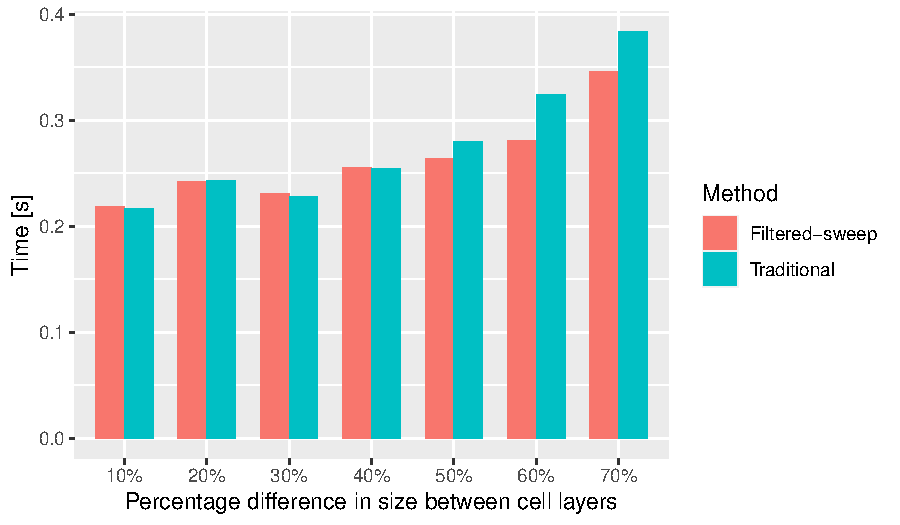
\includegraphics[width=0.48\linewidth]{figures/experiments/Unbalance_Tester02}
    } 
    \caption{Evaluation of the unbalanced layers optimization.}
    \label{fig:unbalance_tests}
\end{figure*}

We also performed an experiment where the difference in size between the two layers varies between 10\% and 70\%. 
For this experiment we first identified cells from the GADM dataset where the smaller layer had around 3K edges. Among these cells we then identified those where the larger layer had 10\%, 20\%, ... up to 70\% more edges. In each category we picked 10 representative cells and computed the overlay for the cells in that category.
Figure \ref{fig:unbalance_b} shows the results; in each category we show the average time to compute the overlay among the 10 cells in that category. 
The filtered-sweep approach shows again better performance as the percentage difference between layers increases. 
Based on these results, one could apply the optimization on those cells where the layer difference is significant (more than 50\%).

\subsection{Varying the number of cells}
The quadtree settings allow for tuning its performance by providing the \textit{number of leaf cells} to be created as a parameter. The quadtree then continues its splits so as to reach this capacity (approximately). The number of cells affects the performance of our scalable overlay implementation (termed as SDCEL below) since it relates to the average cell capacity (in number of edges). 
Fewer number of cells implies larger cell capacity (and thus more edges to process within each cell). On the other hand, creating more cells increases the number of jobs to be executed. 
Figure \ref{fig:ca_a} shows the SDCEL performance using the two layers of the CCT dataset, while varying the number of cells from 100 to 15K (by multiple of 1000). 
Each bar corresponds to the time taken to create the DCEL for each layer and then combining them to create the distributed overlay. 
Clearly there is a trade-off: as the number of cells increases the SDCEL performance improves until a point where the larger number of cells adds an overhead.   
Figure \ref{fig:ca_b} focuses on that area; the best SDCEL performance was around 7K cells.

In addition Figure \ref{fig:ca_a} shows the performance of the sequential solution (CGAL library) for computing the overlay of the two layers in the CCT dataset, using one of the cluster nodes. 
Clearly, the scalable approach is much more efficient as it takes advantage of parallelism. Note that the CGAL library would crash when processing the larger datasets (MainUS and GADM).

\begin{figure*}
    \centering
    \subfloat[ \label{fig:ca_a}]{ 
        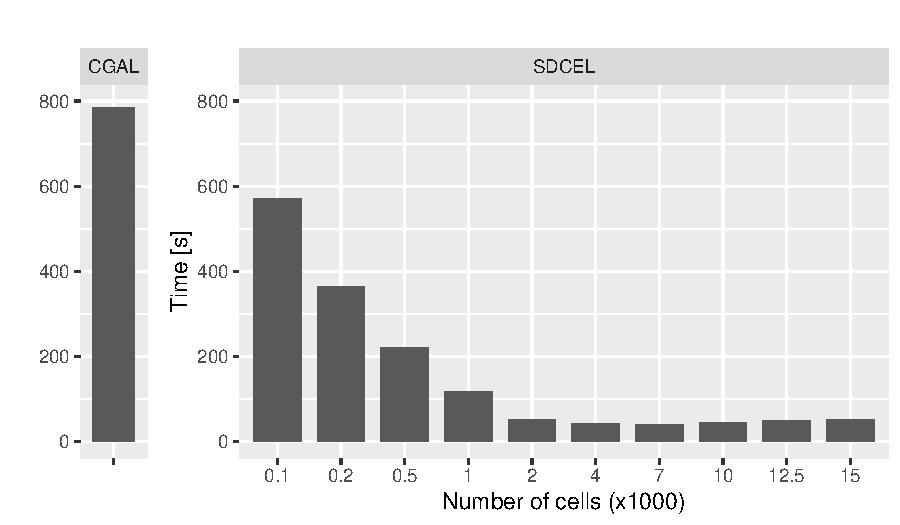
\includegraphics[width=0.75\textwidth]{figures/experiments/CA}
    } \\%\hspace{1cm}
    \subfloat[ \label{fig:ca_b}]{%
        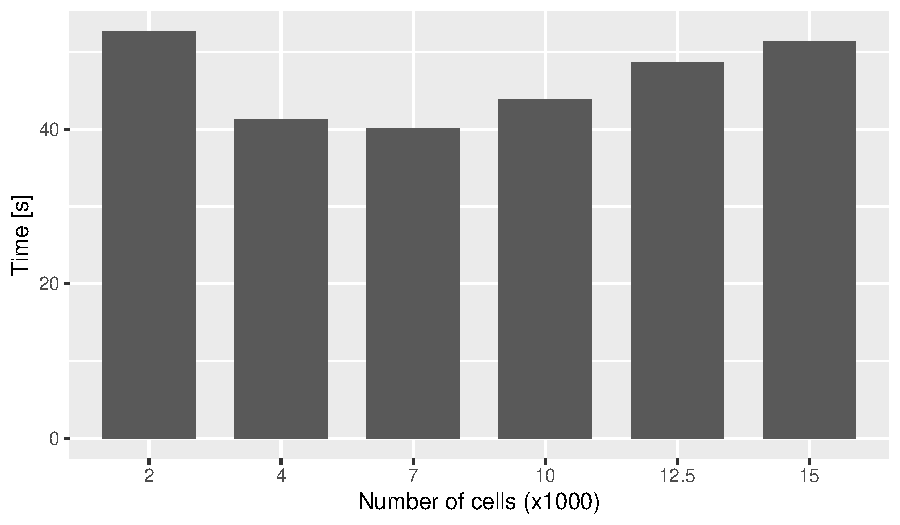
\includegraphics[width=0.75\textwidth]{figures/experiments/CA_sample}
    }
    \caption{SDCEL performance while varying the number of cells in the CCT dataset.} \label{fig:ca}
\end{figure*}

\begin{figure*}
    \centering

    \subfloat[ \label{fig:mainus_a}]{ 
        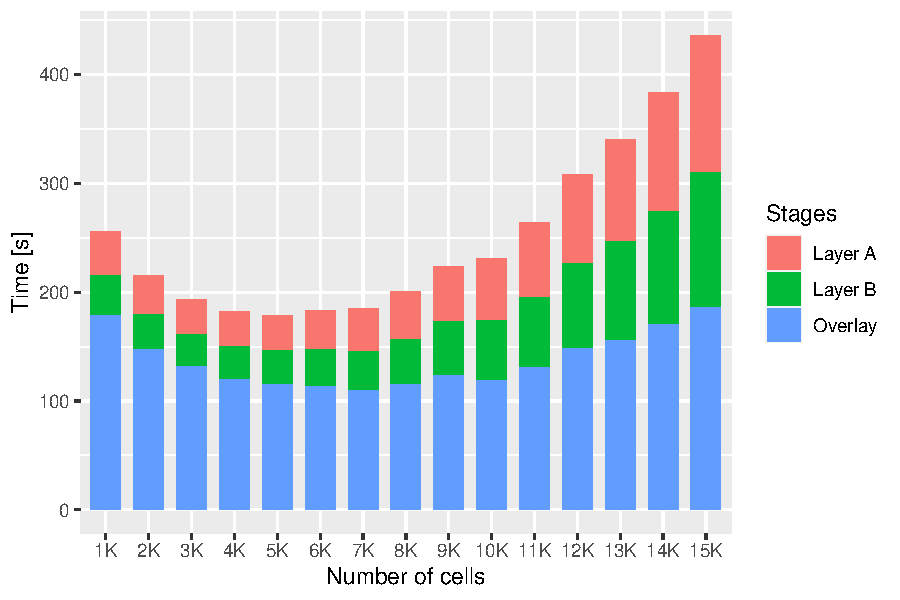
\includegraphics[width=0.75\textwidth]{figures/experiments/MainUS2}
    } \\%\hspace{1cm}
    \subfloat[ \label{fig:gadm_b}]{%
        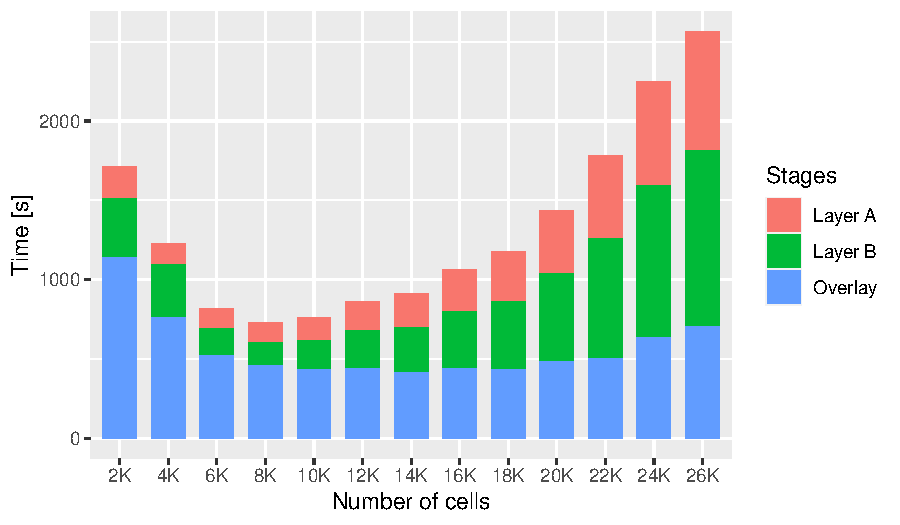
\includegraphics[width=0.75\textwidth]{figures/experiments/GADM2}
    }
    \caption{Performance with (a) MainUS and (b) GADM datasets.} \label{fig:mainus}
\end{figure*}

Figure \ref{fig:mainus} shows the results when using the larger MainUS and GADM datasets, while again varying the number of cells parameter (from 1K to 15K and from 2K to 26K respectively). In this figure we also show the time taken by each stage of the overlay computation (namely, to create the DCEL for layer A, for layer B and for their combination to create their distributed overlay). 
We can see a similar trade-off in each of the stages.  The best performance is given when setting the number of cells parameter to 5K for the MainUS and respectively 8K  for the GADM dataset.  
Note that in the MainUS dataset the two layers have similar number of edges; as it can be seen their DCEL computations are similar. 
Interestingly, the overlay computation is expensive since (as mentioned earlier) there are many intersections between the two layers.
An interesting observation from the GADM plots is that layer B takes more time than layer A; this is because there are more edges in the counties than the states. Moreover, county polygons are included in the (larger) state polygons. 
When the size of cells is small (i.e. larger number of cells like in the case of 26K cells) these cells mainly contain counties from layer B. As a result, there are not many intersections between the layers in each cell and the overlay computation is thus faster. 
On the other hand, with large cell sizes (smaller number of cells) the area covered by the cell is larger, containing more edges from states and thus increase the number of intersections, resulting in higher overlay computation.

\subsection{Speed-up and Scale-up experiments}

The speed-up behavior of SDCEL appears in Figure \ref{fig:mainus_speedup} (for the MainUS dataset) and in Figure \ref{fig:gadm_speedup} (for the GADM dataset); in both cases we show the performance for each stage. For these experiments we varied the number of nodes from 3 to 12 (while keeping the input layers the same).
Clearly, as the number of nodes increases the performance improves. 
SDCEL shows good speed-up characteristics: as the number of nodes doubles (from 3 to 6 and then from 6 to 12) the performance improves almost by half. 

\begin{figure*}
    \centering
    \subfloat[\label{fig:mainus_speedup}]{%
        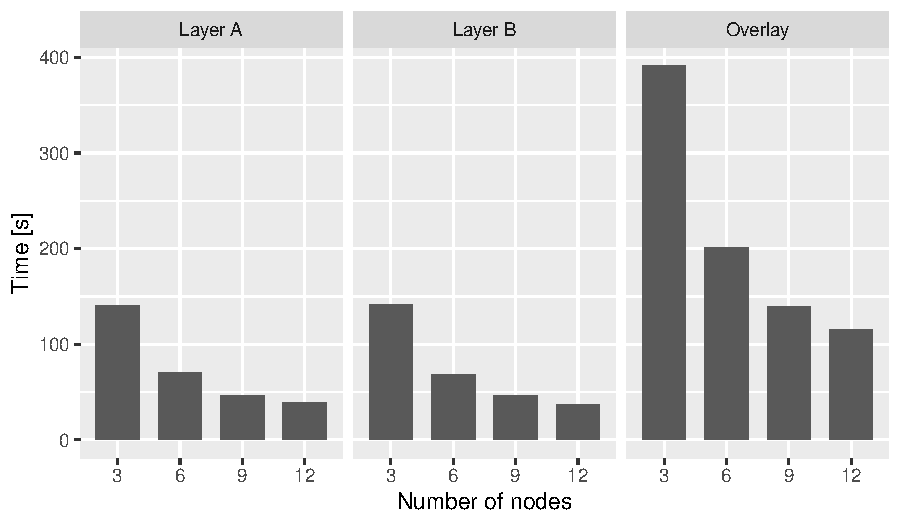
\includegraphics[width=0.75\textwidth]{figures/experiments/MainUS_speedup}
    } \\%\hspace{1cm}
    \subfloat[\label{fig:mainus_scaleup}]{%
        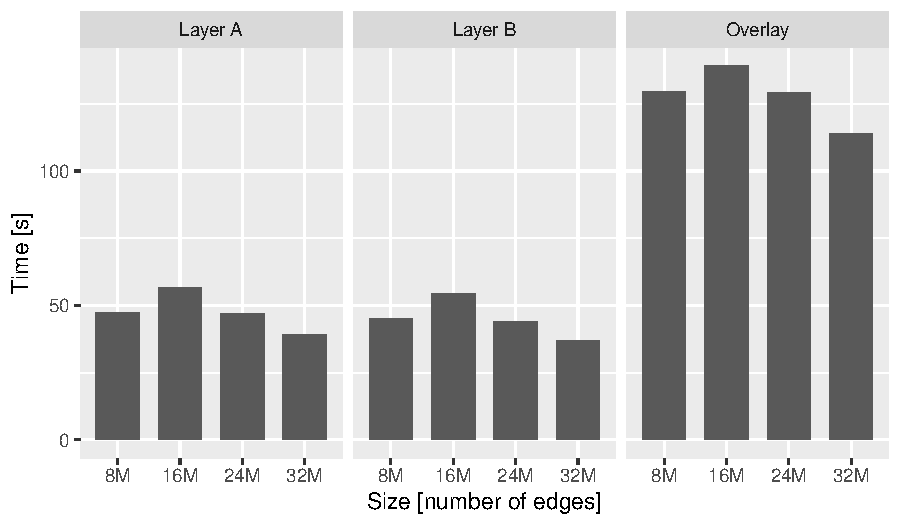
\includegraphics[width=0.75\textwidth]{figures/experiments/MainUS_scaleup}
    }
    \vspace{-10pt}
    \caption{Speed-up and Scale-up experiments for the MainUS dataset.} \label{fig:mainus_speed_scale}
\end{figure*}

\begin{figure*}
    \centering
    \subfloat[\label{fig:gadm_speedup}]{%
        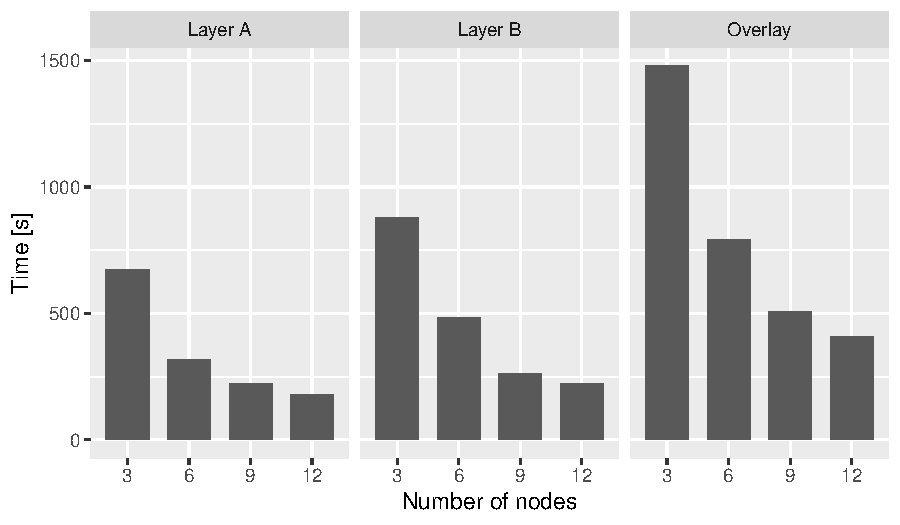
\includegraphics[width=0.75\textwidth]{figures/experiments/GADM_speedup}
         \vspace{-5pt}
    } \\%\hspace{1cm}
    \subfloat[\label{fig:gadm_scaleup}]{%
        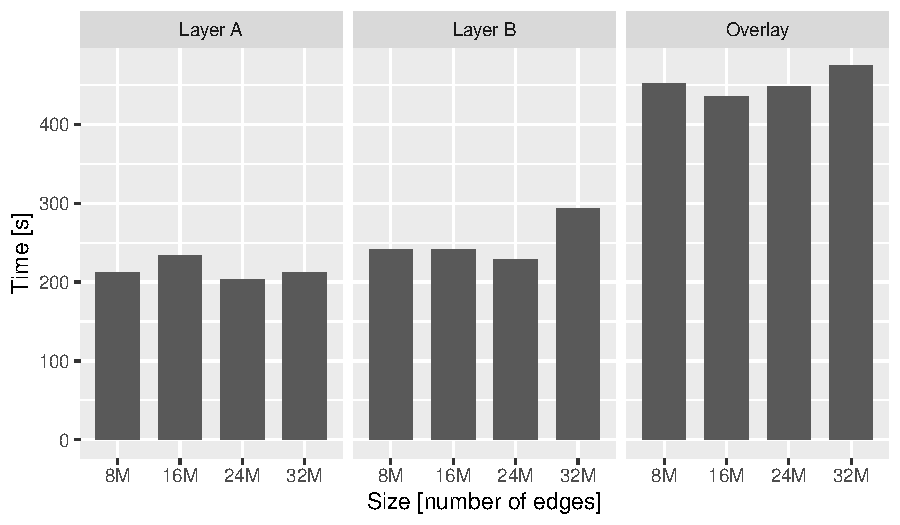
\includegraphics[width=0.75\textwidth]{figures/experiments/GADM_scaleup}
         \vspace{-5pt}
    }
     \vspace{-10pt}
    \caption{Speed-up and Scale-up experiments for the GADM dataset.} \label{fig:gadm_speed_scale}
\end{figure*}

To examine the scale-up behavior we created smaller datasets out of the MainUS (and similarly out of the GADM) so that we can control the number of edges. 
To create such a dataset we picked a centroid and started increasing the area covered by this dataset until the number of edges were closed to a specific number. For example, from the MainUS we created datasets of sizes 8M, 16M, 24M and 32M edges for each layer. We then used two layers of the same size as input to different number of nodes, while keeping the input to node ratio fixed. That is, the layers of size 8M were processed using 3 nodes, the layers of size 16M using 6 nodes, the 24M using 9 nodes and the 32M using 12 nodes. We did the same process for the scale-up experiments of the GADM dataset. The results appear in Figure \ref{fig:mainus_scaleup} and Figure\ref{fig:gadm_scaleup}.
Overall, SDCEL shows good scale-up performance; it remains almost constant as the work per node is similar (there are slight variations because we could not control perfectly the number of edges and their intersection). 

